% =============================================================================
%  PFE Combat Mirror - Rapport d'avancement n°1 : installation de RT-COSMIK
%  Compilation : pdflatex main.tex (x2)   ou   latexmk -pdf main.tex   (ou Overleaf)
% =============================================================================
\documentclass[11pt,a4paper]{article}

\usepackage[utf8]{inputenc}
\usepackage[T1]{fontenc}
\IfFileExists{lmodern.sty}{\usepackage{lmodern}}{}
\IfFileExists{french.ldf}{\usepackage[french]{babel}}{\usepackage[english]{babel}}
\usepackage[margin=2.3cm]{geometry}
\usepackage{graphicx}
\usepackage{booktabs}
\usepackage{float}
\usepackage{tabularx}
\usepackage{array}
\usepackage{amsmath}
\usepackage[table]{xcolor}
\usepackage{listings}
\usepackage[most]{tcolorbox}
\usepackage{enumitem}
\usepackage{fancyhdr}
\usepackage{caption}
\usepackage{csquotes}
\usepackage[hidelinks]{hyperref}

\definecolor{bleu}{HTML}{2a78d6}
\definecolor{orange}{HTML}{eb6834}
\definecolor{encre}{HTML}{3a3a38}
\definecolor{fond}{HTML}{f5f4ef}
\definecolor{vert}{HTML}{1b7a3a}

\hypersetup{colorlinks=true,linkcolor=bleu,urlcolor=bleu,citecolor=bleu}

\lstset{
  basicstyle=\ttfamily\footnotesize,
  backgroundcolor=\color{fond},
  frame=single, rulecolor=\color{fond},
  breaklines=true, breakatwhitespace=false,
  columns=fullflexible, keepspaces=true,
  showstringspaces=false,
  xleftmargin=4pt, xrightmargin=4pt,
  literate={é}{{\'e}}1 {è}{{\`e}}1 {à}{{\`a}}1 {ç}{{\c{c}}}1 {ê}{{\^e}}1 {ù}{{\`u}}1 {ô}{{\^o}}1 {î}{{\^i}}1
}

% Encadré "problème rencontré"
\newtcolorbox{probleme}[1]{enhanced, breakable, colback=white, colframe=orange!80!black,
  boxrule=0.6pt, arc=2pt, left=6pt, right=6pt, top=4pt, bottom=4pt,
  title={\textbf{Problème --} #1}, coltitle=white, colbacktitle=orange!85!black, fonttitle=\small}
\newcommand{\symptome}[1]{\par\noindent\textbf{Symptôme.} #1}
\newcommand{\cause}[1]{\par\smallskip\noindent\textbf{Cause.} #1}
\newcommand{\solution}[1]{\par\smallskip\noindent\textbf{Solution.} #1}

\newcommand{\code}[1]{\texttt{\small #1}}
\newcommand{\acompleter}[1]{\textcolor{orange!85!black}{[À compléter : #1]}}

\pagestyle{fancy}
\fancyhf{}
\lhead{\small PFE Combat Mirror}
\rhead{\small Rapport d'avancement n°1}
\cfoot{\small\thepage}
\renewcommand{\headrulewidth}{0.4pt}

\setlist{itemsep=2pt, topsep=4pt}
\setlength{\emergencystretch}{4em}

\title{\vspace{-1cm}
  \textbf{Instrumentation d'un miroir de boxe Combat Mirror}\\[4pt]
  \large Rapport d'avancement n°1 : installation de RT-COSMIK\\ et première chaîne de capture de mouvement}
\author{Aymeric Duchene\\ \small Polytech Montpellier, département MEA\\
  \small en collaboration avec CSULB (Biomedical Engineering), Combat Mirror et le LAAS-CNRS (Gepetto)}
\date{27 septembre 2026, complété le 28 septembre 2026}

\begin{document}
\maketitle
\thispagestyle{fancy}

\begin{abstract}
Ce document retrace la mise en place du premier livrable du projet : l'installation de RT-COSMIK, la boîte à outils du LAAS qui estime en temps réel la cinématique articulaire d'une personne filmée par des caméras RGB. Il décrit l'environnement de départ, chaque problème rencontré et sa solution, la configuration de la caméra, les scripts développés, et une première évaluation quantitative sur une prise de boxe de 80~s. À la date du rapport, la chaîne complète (caméra $\rightarrow$ détection $\rightarrow$ squelette $\rightarrow$ modèle biomécanique $\rightarrow$ angles articulaires en CSV) fonctionne avec une seule webcam, à environ 15 à 22 résultats par seconde sur le PC Windows. Le 28/09, l'installation a été portée sur la machine Debian de Polytech : après correction d'une incompatibilité entre TensorRT et le driver NVIDIA, la chaîne y traite toutes les images d'une webcam à 30~images/s (54 itérations/s possibles), avec un affichage en direct de la caméra synchronisé avec le squelette 3D.
\end{abstract}

\tableofcontents
\newpage

% =============================================================================
\section{Contexte et objectifs}
% =============================================================================

Le projet vise à instrumenter un miroir d'entraînement de boxe fabriqué par l'entreprise australienne Combat Mirror. Des capteurs de pression placés à l'arrière du miroir doivent mesurer l'intensité et la localisation des impacts. Ces données sont synchronisées avec la cinématique articulaire du boxeur, capturée par deux caméras RGB et le logiciel RT-COSMIK développé au LAAS (Toulouse). Une analyse par IA (par exemple un Transformer) doit ensuite évaluer la séance et produire un score.

\begin{table}[H]
\centering
\begin{tabular}{@{}clp{8.2cm}@{}}
\toprule
& \textbf{Livrable} & \textbf{État au 28/09/2026} \\
\midrule
1 & Installation de RT-COSMIK & \textcolor{vert}{\textbf{Fonctionnel}} avec une webcam : chaîne complète jusqu'aux angles articulaires en CSV, sur le PC Windows puis sur la machine Debian de Polytech en temps réel à 30~images/s (objet de ce rapport). \\
2 & Instrumentation du miroir & Non commencé. \\
3 & Synchronisation et CSV & Côté caméra prêt : CSV horodatés par compteur d'images. \\
4 & Algorithme de traitement (IA) & Non commencé, dépend du livrable 3. \\
\bottomrule
\end{tabular}
\caption{Avancement des livrables.}
\end{table}

\paragraph{Ressources fournies par le LAAS.}
Le code de RT-COSMIK est public sur le GitHub de l'équipe Gepetto : \url{https://github.com/Gepetto/rt-cosmik}. La branche \code{offline-paper}, indiquée comme la plus à jour, a été fusionnée dans \code{main} le 22/09/2026 (commit \code{064353f}). S'y ajoutent l'outil de calibration \url{https://github.com/Gepetto/cams_calibration}, un pont ROS~2 \url{https://github.com/Gepetto/rtcosmik_ros}, et un conteneur Docker de développement \url{https://github.com/MaximeSabbah/cosmik-dev-container}. Les caméras utilisées nativement par le LAAS sont des webcams Creative à bas coût.

% =============================================================================
\section{Point de départ et environnement}
% =============================================================================

\subsection{Première tentative sur MacBook}

La première tentative a consisté à cloner RT-COSMIK sur un MacBook Pro et à lancer \code{./scripts/bash/fetch\_models.sh}, qui télécharge les poids des modèles.

\begin{probleme}{Téléchargement des modèles impossible sur macOS}
\symptome{\code{ssl.SSLCertVerificationError: [SSL: CERTIFICATE\_VERIFY\_FAILED] unable to get local issuer certificate} lors de l'appel \code{urllib} du script.}
\cause{Le Python 3.11 installé depuis python.org (\code{/Library/Frameworks/Python.framework}) n'utilise pas les certificats du système. Son paquet de certificats doit être installé séparément.}
\solution{Exécuter \code{/Applications/Python 3.11/Install Certificates.command} (installe \code{certifi}), puis vérifier avec \code{urllib.request.urlopen('https://github.com')}.}
\end{probleme}

RT-COSMIK s'appuie sur CUDA et TensorRT (moteurs de détection YOLO, modèle NLF sur GPU), ce qui exige un GPU NVIDIA. Le travail s'est donc poursuivi sur un PC Windows équipé d'une carte graphique NVIDIA, dans le conteneur Docker fourni par le LAAS.

\subsection{Environnement retenu}

\begin{table}[H]
\centering
\begin{tabularx}{\textwidth}{@{}lX@{}}
\toprule
\textbf{Élément} & \textbf{Valeur} \\
\midrule
Hôte & Windows, Docker Desktop (moteur WSL~2), \code{usbipd} pour partager l'USB avec WSL \\
GPU & NVIDIA GeForce RTX 4070 SUPER, 12~Go, compute capability 8.9 \\
Image Docker & \code{mmpose\_image}, construite depuis le \code{Dockerfile} de \code{cosmik-dev-container} \\
Base de l'image & \code{nvidia/cuda:12.1.1-cudnn8-devel-ubuntu22.04} (Ubuntu 22.04, Python 3.10) \\
Bibliothèques & torch 2.4.1+cu121, torchvision 0.19.1+cu121, TensorRT 11.3.0, NumPy 1.26.4 (épinglé), ROS~2 Humble ; compilés depuis les sources : Pinocchio 3.9.0 (avec CasADi), CasADi 3.7.2, coal 3.0.2, eigenpy 3.12, FATROP, acados, example-robot-data \\
RT-COSMIK & Préinstallé : \code{MaximeSabbah/RT-COSMIK}, branche \code{main}, commit \code{bd80b0d} (identique à la branche \code{nlf\_humble} de Gepetto). Ajouté : \code{Gepetto/rt-cosmik}, branche \code{main}, commit \code{064353f} \\
Caméra & Webcam UGREEN (USB \code{0c45:2283}), une seule pour l'instant \\
\bottomrule
\end{tabularx}
\caption{Environnement matériel et logiciel. Le relevé exact des versions est produit par \code{scripts/tools/collect\_from\_container.sh} (\code{docs/container\_versions.txt}).}
\end{table}

Le conteneur n'a pas de dossier partagé avec Windows : tous les fichiers de travail vivent à l'intérieur (\code{/root/workspace/ros\_ws/}) et sont récupérés avec \code{docker cp}. Des instantanés ont été pris avec \code{docker commit} (\code{cosmik-backup:2026-09-26}, puis après la démonstration). La construction de l'image et l'installation complète sont décrites dans \code{docs/SETUP.fr.md}.

% =============================================================================
\section{Architecture de RT-COSMIK}
% =============================================================================

La lecture du code de la branche \code{main} donne la chaîne de traitement suivante, pour chaque itération :

\begin{enumerate}
  \item \textbf{Acquisition} : un processus par caméra lit le flux MJPEG de \code{/dev/video<i>} via \textbf{ffmpeg}, et non OpenCV, pour limiter la latence et enregistrer la vidéo sans ré-encodage. Une barrière synchronise les caméras.
  \item \textbf{Détection} : YOLOv10n, sous forme de moteur TensorRT, localise la personne. Le moteur est construit avec une taille de lot fixe égale au nombre de caméras (\code{yolov10n\_b<N>.engine}).
  \item \textbf{Estimation de pose} : NLF (\emph{Neural Localizer Fields}, modèle TorchScript \code{nlf\_s\_multi\_0.2.2}) prédit, dans la boîte détectée, la position 2D/3D de 43 points choisis sur le maillage SMPL-X. Ces points jouent le rôle de marqueurs anatomiques virtuels (épines iliaques, C7, épaules, épicondyles, poignets, genoux, chevilles, pieds, tête).
  \item \textbf{Reconstruction 3D} : NLF fournit pour chaque caméra une pose 3D métrique, dans le repère de cette caméra, avec une incertitude par point. Les poses des différentes caméras sont fusionnées, pondérées par l'inverse de leur incertitude. Avec une seule caméra, on garde son estimation monoculaire, dont la profondeur est moins précise. Les points sont ensuite exprimés dans le repère monde ($p_\text{monde} = R\,p_\text{caméra} + T$), puis lissés par un filtre passe-bas de Butterworth d'ordre~4 (coupure 10~Hz).
  \item \textbf{Modèle biomécanique} : un modèle humain multicorps (example-robot-data, Pinocchio) est mis à l'échelle du sujet (taille, masse) sur les premières images, pendant lesquelles le sujet reste immobile.
  \item \textbf{Cinématique inverse contrainte} : à chaque image, on cherche la configuration articulaire $q$ qui minimise l'écart entre les marqueurs du modèle et les marqueurs mesurés, sous contraintes (limites articulaires, segments rigides). Deux solveurs existent : \code{sbs} (programme quadratique image par image, quadprog) et \code{mhe} (estimation sur horizon glissant, acados ou FATROP, à précompiler).
  \item \textbf{Sorties} : \code{joint\_angles.csv} (position et orientation du bassin, puis 36 angles articulaires en radians), \code{markers.csv} (43 marqueurs en 3D, en mètres), la vidéo \code{camera\_<i>.mkv}, une visualisation 3D Meshcat dans le navigateur et, depuis le patch \code{0003} (section~\ref{sec:debian}), une fenêtre montrant l'image de la caméra avec les points NLF.
\end{enumerate}

% =============================================================================
\section{Chronologie de l'installation : problèmes et solutions}
% =============================================================================

\subsection{Moteur TensorRT de YOLO (26/09)}

Le moteur de détection a été généré avec \code{yolo export} (\code{.pt} $\rightarrow$ ONNX $\rightarrow$ TensorRT 11.3), en lot de 2 (\code{yolov10n\_b2\_img640\_fp32.engine}, 138~Mo) puis de 1 (\code{yolov10n.engine}, 91~Mo).

\begin{probleme}{Le moteur généré est refusé par TensorRT}
\symptome{\code{trtexec -{}-loadEngine=weights/yolo/yolov10n.engine} échoue : \code{Serialization assertion header.magicTag == kEXPECTED\_MAGIC\_TAG failed ... incompatible serialization version (1875 != 1953657958)}, alors que \code{trtexec} et le module Python sont tous deux en TensorRT 11.3.0.}
\cause{L'examen des premiers octets (\code{xxd}) montre \code{53 07 00 00 7b 22 64 65 73 63...}, soit un entier de 4 octets ($\mathtt{0x753} = 1875$) suivi d'un JSON \code{\{"description": "Ultralytics YOLOv10n model...}. Ultralytics préfixe le moteur TensorRT brut par ses propres métadonnées. TensorRT lit donc 1875 là où il attend sa signature $\mathtt{0x74727466}$ (\enquote{ftrt} = 1953657958).}
\solution{Aucune conversion n'est nécessaire. RT-COSMIK charge le détecteur avec \code{ultralytics.YOLO(chemin, task="detect")}, qui sait lire ce format. Le script \code{scripts/tests/engine\_metadata.py} lit ces métadonnées ; le moteur batch 1 est bien en \code{batch 1, imgsz [640, 640]}. \textbf{Leçon} : lire le code du chargeur avant de déboguer le format d'un fichier.}
\end{probleme}

\subsection{Mise en service de la webcam (26/09)}

La webcam est partagée de Windows vers WSL~2 avec \code{usbipd attach -{}-wsl -{}-busid 5-2} et apparaît dans le conteneur comme \code{/dev/video0} (bus \code{usb-vhci\_hcd.0-1}, c'est-à-dire USB/IP). Le premier test (\code{scripts/tests/test\_webcam.py}) confirme la capture et la détection d'une personne par YOLO, mais à seulement \textbf{2,0~images/s} en 1280$\times$720.

\begin{probleme}{Cadence de la caméra très faible}
\symptome{2~fps mesurés avec OpenCV en 1280$\times$720 pour une caméra annoncée à 30~fps.}
\cause{Deux causes cumulées, isolées avec \code{v4l2-ctl -{}-stream-mmap} :
\begin{itemize}
  \item le réglage \code{exposure\_dynamic\_framerate} était à 1 (défaut constructeur : 0). La caméra baisse alors sa cadence pour allonger l'exposition dès que la lumière faiblit. Un test capuchon fermé l'a confirmé : les fps chutent puis remontent avec la lumière ;
  \item une fois ce réglage corrigé, la cadence reste plafonnée et \emph{parfaitement stable} : 3,7~fps en 1280$\times$720 et environ 13~fps en 640$\times$480. Diviser le nombre de pixels par 3 multiplie les fps par 3,5 : c'est une limite de bande passante du transport USB/IP de WSL, qui gère mal les transferts isochrones des webcams.
\end{itemize}}
\solution{\code{v4l2-ctl -d /dev/video0 -c exposure\_dynamic\_framerate=0} à chaque branchement, et passage du pipeline en \textbf{640$\times$480}. La solution définitive est un Linux natif (machine Debian de Polytech), où la caméra est vue directement, sans USB/IP.}
\end{probleme}

\subsection{Premier squelette par IA (26/09)}

Le modèle NLF a été testé seul sur une photo prise par la webcam (script \code{test\_skeleton\_nlf.py}, méthode \code{detect\_smpl\_batched}, 24 articulations SMPL). La figure~\ref{fig:nlf} montre le résultat, sujet en garde. Le bassin, la colonne, les coudes, les poings et les jambes sont bien placés. Les épaules sont légèrement ramenées vers l'intérieur, car elles sont masquées par les bras en garde de face. Les pieds sont hors champ.

\begin{figure}[H]
\centering
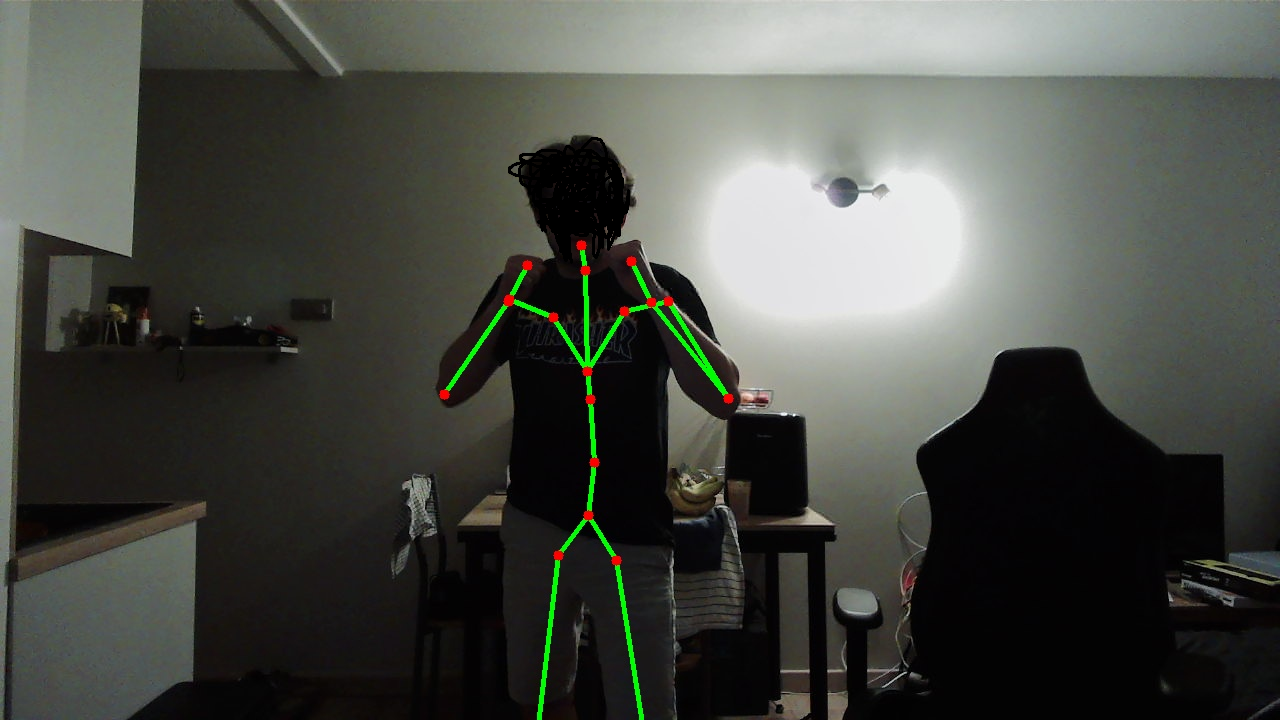
\includegraphics[width=0.62\textwidth]{figures/squelette_nlf_debout.png}
\caption{Squelette 2D estimé par NLF sur une image de la webcam (1280$\times$720), sujet en garde de boxe.}
\label{fig:nlf}
\end{figure}

\subsection{Choix de la version de RT-COSMIK (27/09)}

\begin{probleme}{La version préinstallée ne gère pas une seule caméra}
\symptome{Le dossier \code{config/cam\_params} est vide, et la branche préinstallée (\code{bd80b0d}) attend des fichiers de calibration aux noms fixes.}
\cause{Dans cette version, \code{load\_camera\_parameters} charge toujours au moins deux caméras (\code{c0\_params\_color.yaml}, \code{c2\_params\_color.yaml} et leur pose relative), et le pipeline triangule systématiquement.}
\solution{Installation de la branche \code{main} de Gepetto (\code{064353f}) \emph{à côté} de l'existante (\code{RT-COSMIK-main}), pour ne rien casser. Cette version accepte \code{-{}-cameras 0} (NLF monoculaire), ne demande que les intrinsèques \code{config/cam\_params/intrinsics/camera\_0\_intrinsics.yaml}, et choisit le moteur YOLO selon le nombre de caméras. Poids réutilisés, moteur batch~1 renommé \code{yolov10n\_b1.engine} avec un fichier \code{.meta} contenant \code{1,640} ; ffmpeg installé.}
\end{probleme}

Les réglages modifiés dans \code{settings.py} sont regroupés dans le tableau~\ref{tab:settings} (patch \code{rtcosmik/patches/0002-settings-single-webcam.patch}).

\begin{table}[H]
\centering
\begin{tabular}{@{}lllp{5.6cm}@{}}
\toprule
\textbf{Paramètre} & \textbf{Défaut} & \textbf{Utilisé} & \textbf{Raison} \\
\midrule
\code{width, height} & 1280$\times$720 & 640$\times$480 & Bande passante USB/IP (13 contre 3,7~fps) \\
\code{fs} & 40 & 30 & Maximum de la webcam \\
\code{cameras} & (0, 2, 4, 6) & (0,) & Une seule webcam \\
\code{ik\_type} & \code{mhe} & \code{sbs} & Aucun solveur à précompiler \\
\code{human\_height/weight} & 1,80~m, 70~kg & 1,73~m, 67~kg & Mise à l'échelle du modèle \\
\code{no\_trial} & \code{test} & \code{demo\_0X} & Un dossier de sortie par prise \\
\bottomrule
\end{tabular}
\caption{Réglages de RT-COSMIK modifiés.}
\label{tab:settings}
\end{table}

\subsection{Calibration intrinsèque sans damier imprimé (27/09)}

Faute d'imprimante (week-end), le damier (10$\times$7 cases, soit 9$\times$6 coins intérieurs) a été affiché en plein écran sur un ordinateur portable, luminosité maximale. Un écran est parfaitement plan, ce qui convient bien à la calibration. Le script \code{scripts/calibration/calib\_intrinsics.py} capture 25 vues où le damier est détecté, puis estime le modèle sténopé avec distorsion radiale et tangentielle :
\begin{equation}
s\begin{pmatrix}u\\v\\1\end{pmatrix} = K \begin{pmatrix}x_d\\y_d\\1\end{pmatrix},\qquad
K = \begin{pmatrix} f_x & 0 & c_x\\ 0 & f_y & c_y\\ 0&0&1\end{pmatrix},\qquad
D = (k_1, k_2, p_1, p_2, k_3),
\end{equation}
où $(x_d, y_d)$ sont les coordonnées normalisées après distorsion.

\begin{probleme}{Erreur de reprojection élevée}
\symptome{Premier calcul : RMS de 4,44~px (objectif $< 1$), $f_x = 381{,}6$ et $f_y = 392{,}3$ (écart de 3~\% suspect pour des pixels carrés).}
\cause{La fenêtre d'affinement sous-pixel des coins (\code{cornerSubPix}) était de 11$\times$11~px. En 640$\times$480, les cases du damier sont petites à l'image : la fenêtre débordait sur les cases voisines et déplaçait les coins.}
\solution{Recalcul sur les \emph{mêmes} 25 images avec une fenêtre 5$\times$5 (\code{scripts/calibration/recalib.py}, qui écarte aussi itérativement les pires vues si nécessaire) : \textbf{RMS de 0,67~px}, $f_x \approx f_y$ à 0,4~\% près. La première focale était fausse de 23~\%. Le script de capture utilise désormais 5$\times$5.}
\end{probleme}

\begin{table}[H]
\centering
\begin{tabular}{@{}lr@{\hspace{2em}}lr@{}}
\toprule
\multicolumn{2}{@{}l}{\textbf{Intrinsèques} (640$\times$480)} & \multicolumn{2}{l@{}}{\textbf{Distorsion}} \\
\midrule
$f_x$ & 492,57~px & $k_1$ & $-0{,}0690$ \\
$f_y$ & 494,71~px & $k_2$ & $0{,}1739$ \\
$c_x$ & 361,45~px & $p_1$ & $-0{,}0028$ \\
$c_y$ & 228,56~px & $p_2$ & $0{,}0327$ \\
RMS & 0,673~px & $k_3$ & $-0{,}0909$ \\
\bottomrule
\end{tabular}
\caption{Calibration retenue (\code{config/cam\_params/intrinsics/camera\_0\_intrinsics.yaml}). Champ de vision : $2\arctan(320/f_x) = 66{,}0^\circ$ en horizontal, $51{,}8^\circ$ en vertical.}
\label{tab:calib}
\end{table}

Point à reprendre : le centre optique est décalé de 41~px vers la droite par rapport au centre de l'image, et le coefficient tangentiel $p_2$ est relativement élevé. Ces deux paramètres sont corrélés, et ce décalage est typique de vues qui ne couvrent pas assez les bords de l'image (en particulier le bord gauche). Une nouvelle capture insistant sur les coins est prévue.

\subsection{Premier lancement du pipeline complet (27/09)}

\begin{probleme}{Plantage au chargement de NLF}
\symptome{\code{RuntimeError: Unknown builtin op: torchvision::nms} dans le processus pipeline ; les processus caméra restent bloqués à la barrière.}
\cause{Le modèle NLF (TorchScript) appelle l'opérateur \code{torchvision::nms}, qui n'est enregistré dans PyTorch que si \code{torchvision} a été importé. \code{src/rtcosmik/nlf/nlf.py} ne l'importe pas, et le processus est lancé en mode \code{spawn}, donc sans hériter des imports du processus parent.}
\solution{Ajout de \code{import torchvision} en tête de \code{nlf.py} (patch \code{rtcosmik/patches/0001-nlf-import-torchvision.patch}). \textbf{Modification à signaler au LAAS.}}
\end{probleme}

Après correction, le pipeline démarre, calibre le modèle sur le sujet, puis tourne à \textbf{22~itérations/s} (boucle de 45~ms, dont 41~ms pour l'estimation de pose et 2,8~ms pour la cinématique inverse). Les messages restants sont sans gravité : conflit de version SciPy/NumPy système, avertissement \code{'half' is deprecated} d'Ultralytics (masqué par \code{export YOLO\_VERBOSE=False}), et absence de repère monde (les positions sont exprimées dans le repère de la caméra ; les angles articulaires n'en dépendent pas).

\subsection{Visualisation et synchronisation vidéo / CSV (27/09)}

La version \code{main} n'ouvre pas de fenêtre vidéo : la seule visualisation en direct est Meshcat (serveur web sur le port 7000 du conteneur), qui doit être redirigé vers Windows (redirection de port VS Code). Pour obtenir une démonstration lisible, le script \code{scripts/analysis/overlay\_video.py} projette les marqueurs 3D de \code{markers.csv} sur la vidéo enregistrée à l'aide de $K$ et $D$, et affiche les angles des coudes.

\begin{probleme}{Squelette décalé par rapport à la vidéo}
\symptome{Premier essai : aucun squelette dessiné. Deuxième : squelette très en retard (environ 20~s). Prise \code{demo\_02} : compteur CSV de 586 à 2231 pour seulement 473 images dans la vidéo.}
\cause{La colonne \code{Frame\_0} compte les images lues par le processus caméra, à environ 30 par seconde. Interprétation : ffmpeg duplique les images pour tenir la cadence demandée, alors que la webcam n'en livre que 6 à 7 réelles via WSL. La vidéo \code{.mkv}, copie directe du flux de la caméra, ne contient que les images réelles, sur toute la durée de la prise. Les 586 premières valeurs du compteur correspondent aux environ 20~s de chargement de NLF et de calibration du sujet, pendant lesquelles aucune ligne n'est écrite.}
\solution{Recaler linéairement le compteur sur la vidéo (compteur 0 = première image, compteur maximal = dernière image), avec un petit décalage réglable \code{OFFSET}. \code{overlay\_offsets.sh} génère une vidéo par valeur de décalage pour choisir la meilleure à l'\oe il. Une synchronisation exacte passera par les horodatages (piste pour le livrable~3). Sur \code{demo\_03}, un décalage nul est déjà presque juste, tandis qu'un décalage de +3 images fait précéder la vidéo par le squelette : l'optimum se situe autour d'une image (environ 0,13~s à 7,5 images réelles par seconde). Le décalage accepte donc des valeurs fractionnaires.}
\end{probleme}

\subsection{Portage sur la machine Debian de Polytech (28/09)}
\label{sec:debian}

Pour lever la limite de cadence due à WSL, l'installation a été reprise sur la machine Debian de Polytech, où la webcam est vue directement (\code{/dev/video0}), sans USB/IP. Docker et l'image \code{mmpose\_image} y avaient déjà été préparés.

\begin{table}[H]
\centering
\begin{tabularx}{\textwidth}{@{}lX@{}}
\toprule
\textbf{Élément} & \textbf{Valeur} \\
\midrule
Hôte & Debian, poste \code{tp-autom026} \\
GPU & NVIDIA RTX A1000, 8~Go ; driver 550.163.01 (CUDA 12.4 au maximum) \\
Accès GPU & \code{nvidia-container-toolkit} déjà configuré : \code{nvidia-smi} fonctionne dans un conteneur \code{nvidia/cuda:12.1.1} \\
Image Docker & \code{mmpose\_image:latest}, construite depuis le \code{Dockerfile} de \code{cosmik-dev-container} \\
Conteneur & \code{cosmik}, créé avec \code{-{}-gpus all -{}-privileged -v /dev:/dev -{}-net=host} et l'accès à l'affichage X11 ; relancé ensuite par \code{docker start -ai cosmik} \\
TensorRT & 10.16.1 pour CUDA~12 (pip \code{tensorrt-cu12}), à la place de la 11.3 de l'image \\
Caméra & Webcam USB de Polytech, calibration de la webcam UGREEN utilisée provisoirement \\
\bottomrule
\end{tabularx}
\caption{Environnement de la machine Debian de Polytech.}
\end{table}

\begin{probleme}{TensorRT inutilisable avec le driver de la machine}
\symptome{\code{import tensorrt} fonctionne, mais la création d'un builder échoue : \code{cudaError 35: CUDA driver version is insufficient for CUDA runtime version}, puis \code{createInferBuilder: CUDA initialization failure}. Aucun moteur YOLO ne peut être construit.}
\cause{Le \code{Dockerfile} installe \code{libnvinfer-bin} par apt sans fixer de version. Au moment du build, le dépôt NVIDIA fournissait TensorRT 11.3 compilé pour CUDA~13.4 (paquets \code{11.3.0.99-1+cuda13.4}). CUDA~13 exige un driver 580 ou plus récent, alors que le driver 550 de la machine s'arrête à CUDA~12.4. Le module Python se charge, mais l'initialisation de CUDA échoue.}
\solution{Dans le conteneur, suppression des 7 paquets TensorRT CUDA~13 (\code{apt-get purge}) et installation de \code{tensorrt-cu12} 10.16 par pip. Les versions CUDA~12 fonctionnent avec tout driver à partir de la série 525 (compatibilité mineure de CUDA~12). Vérification : \code{trt.Builder(trt.Logger())} passe, NumPy reste en 1.26.4. La correction a été ajoutée à \code{setup\_rtcosmik\_main.sh} de façon conditionnelle : le script teste d'abord TensorRT et ne le remplace (en supprimant les anciens moteurs, liés à la version de TensorRT qui les a produits) que si le test échoue. Sur une machine où TensorRT fonctionne, rien ne change. \textbf{À signaler au LAAS} : fixer la version de \code{libnvinfer-bin} dans le \code{Dockerfile}.}
\end{probleme}

L'installation s'est ensuite faite en une commande avec \code{setup\_rtcosmik\_main.sh} : clone de \code{Gepetto/rt-cosmik} (\code{064353f}), application des patchs, copie de la calibration, téléchargement des poids NLF et YOLO et export du moteur \code{yolov10n\_b1.engine} en 67~s. Un conteneur trouvé sur la machine (\code{rtcosmik-dev}) était vide et lancé sans \code{-{}-privileged}, donc sans accès à la caméra ; il a été abandonné au profit d'un nouveau conteneur nommé. L'état final est sauvegardé par \code{docker commit cosmik mmpose\_image:rtcosmik-ready}.

\begin{table}[H]
\centering
\begin{tabular}{@{}lrr@{}}
\toprule
\textbf{Étape} & \textbf{Debian, RTX A1000} & \textbf{Windows, RTX 4070 SUPER} \\
\midrule
Estimation de pose (YOLO + NLF) & 14,5~ms & 41~ms \\
Cinématique inverse & 3,0~ms & 2,8~ms \\
Boucle complète & 18,4~ms & 45~ms \\
Itérations par seconde & 54 & 22 \\
Images de la caméra traitées & 100~\% (30~images/s) & 6 à 13~images/s réelles \\
\bottomrule
\end{tabular}
\caption{Temps par itération (médianes). Debian : 385 itérations, avant l'ajout de la fenêtre caméra. Windows : section précédente.}
\label{tab:debian}
\end{table}

La webcam fournit désormais ses 30~images/s et chaque image est traitée : la limite liée à WSL est levée. L'estimation de pose est près de trois fois plus rapide sur la Debian, alors que la carte y est moins puissante ; l'environnement WSL/Docker Desktop est le premier suspect, à confirmer.

\begin{probleme}{Modèle 3D allongé face au sol dans Meshcat}
\symptome{Les points suivent correctement la personne, mais le modèle biomécanique apparaît couché, le visage vers le sol.}
\cause{Sans pose caméra$\rightarrow$monde, le repère de la caméra sert de repère monde. En vision, ce repère a $X$ vers la droite de l'image, $Y$ vers le bas et $Z$ vers l'avant, alors que Meshcat affiche avec $Z$ vers le haut. Les angles articulaires ne sont pas affectés : ils ne dépendent que des positions relatives des marqueurs.}
\solution{Ajout d'une pose caméra$\rightarrow$monde pour la caméra~0, dans le fichier \code{camera\_0\_extrinsics.yaml} du dossier \code{config/cam\_params/extrinsics/}, en supposant la webcam horizontale à 1,2~m du sol :
\begin{equation}
R = \begin{pmatrix} 0 & 0 & 1\\ -1 & 0 & 0\\ 0 & -1 & 0 \end{pmatrix},\qquad
T = \begin{pmatrix} 0\\ 0\\ 1{,}2 \end{pmatrix}\ \text{m},
\end{equation}
soit $X_\text{monde} = Z_\text{caméra}$ (vers l'avant), $Y_\text{monde} = -X_\text{caméra}$, $Z_\text{monde} = -Y_\text{caméra}$ (vers le haut), avec $\det R = 1$. Le modèle est alors debout. Cette pose est approximative ; une calibration extrinsèque (marqueur ArUco) donnera la position réelle. Le script de setup copie ce fichier.}
\end{probleme}

\subsection{Affichage synchronisé caméra et squelette (28/09)}

La visualisation par superposition après coup (\code{overlay\_video.py}) demandait un recalage manuel. Pour une démonstration en direct, le patch \code{rtcosmik/patches/0003-live-camera-overlay.patch} ajoute au processus pipeline une fenêtre OpenCV qui affiche, à chaque itération, l'image de la caméra avec les points 2D de NLF et la boîte de détection (fonction \code{visualize\_frames}, déjà présente dans RT-COSMIK). L'image affichée est exactement celle dont est issu le squelette envoyé à Meshcat dans la même itération : les deux vues sont synchronisées par construction. Le réglage \code{show\_video} de \code{settings.py} permet de désactiver la fenêtre. Sur la Debian, Meshcat est ouvert directement dans Firefox (\code{http://127.0.0.1:7000/static/}), grâce à \code{-{}-net=host}.

\acompleter{capture d'écran de la démonstration : fenêtre caméra et Meshcat côte à côte}

% =============================================================================
\section{Scripts développés}
% =============================================================================

Tous les scripts sont versionnés dans le dépôt \code{pfe-combat-mirror} et se lancent depuis la racine de RT-COSMIK.

\begin{table}[H]
\centering
\small
\begin{tabularx}{\textwidth}{@{}lX@{}}
\toprule
\textbf{Script} & \textbf{Rôle} \\
\midrule
\code{tests/test\_webcam.py} & Ouvre la webcam, mesure les fps réels, détection YOLO sur une image \\
\code{tests/test\_skeleton\_nlf.py} & Photo avec compte à rebours, squelette 2D NLF (24 articulations) \\
\code{tests/test\_yolo\_engine.py} & Vérifie qu'un moteur TensorRT se charge et détecte une personne \\
\code{tests/engine\_metadata.py} & Lit l'en-tête Ultralytics d'un \code{.engine} (lot, taille d'image) \\
\code{calibration/checkerboard\_9x6.png} & Damier à afficher en plein écran \\
\code{calibration/calib\_intrinsics.py} & Capture automatique de vues du damier et calibration \\
\code{calibration/recalib.py} & Recalcul depuis les images enregistrées, rejet des pires vues \\
\code{analysis/analyze\_take.py} & Qualité d'une prise : trous, stabilité des segments, sauts, graphes \\
\code{analysis/overlay\_video.py} & Vidéo avec squelette superposé et angles des coudes \\
\code{analysis/overlay\_offsets.sh} & Une vidéo de superposition par valeur de décalage \\
\code{tools/collect\_from\_container.sh} & Exporte du conteneur config, modifications, résultats et versions \\
\code{tools/setup\_rtcosmik\_main.sh} & Installe RT-COSMIK \code{main}, applique les patchs, copie la calibration et la pose caméra$\rightarrow$monde, remplace TensorRT s'il est incompatible avec le driver, télécharge les modèles \\
\bottomrule
\end{tabularx}
\caption{Scripts du dépôt (dossier \code{scripts/}).}
\end{table}

% =============================================================================
\section{Configuration de la caméra}
% =============================================================================

\begin{table}[H]
\centering
\begin{tabularx}{\textwidth}{@{}lX@{}}
\toprule
Modèle & UGREEN Camera, USB \code{0c45:2283} \\
Formats & MJPG, entre autres 1920$\times$1080, 1440$\times$1080, 1280$\times$960, 1280$\times$720, 1024$\times$768 ; 5 à 30~fps \\
Mode utilisé & MJPG 640$\times$480, 30~fps demandés (environ 6 à 13~fps réels via WSL) \\
Exposition & \code{auto\_exposure = 3} (priorité ouverture), \code{exposure\_dynamic\_framerate = 0} \\
Accès & \code{usbipd attach -{}-wsl -{}-busid 5-2}, puis \code{/dev/video0} dans le conteneur \\
Placement & Face au sujet ; 2,5 à 3~m recommandés (voir section~\ref{sec:resultats}) \\
Calibration & Tableau~\ref{tab:calib} \\
\bottomrule
\end{tabularx}
\caption{Configuration de la webcam.}
\end{table}

% =============================================================================
\section{Premiers résultats : prise \code{demo\_03}}
\label{sec:resultats}
% =============================================================================

Prise d'environ 80~s en direct : immobilité pour la calibration du modèle, garde, puis enchaînements libres de directs et de crochets (le protocole prévu n'a pas été suivi strictement). Le script \code{analyze\_take.py} donne :

\begin{table}[H]
\centering
\begin{tabular}{@{}lrrl@{}}
\toprule
\textbf{Indicateur} & \multicolumn{2}{c}{\textbf{Valeur}} & \textbf{Lecture} \\
\midrule
Lignes / durée / cadence & \multicolumn{2}{r}{1225 / 80,5~s / 15,2~Hz} & \\
Valeurs manquantes & \multicolumn{2}{r}{0~\%} & Aucune perte de suivi \\
\midrule
\textit{Segment} & \textit{médiane} & \textit{variation} & \\
Bras D / G & 31,9 / 33,6~cm & 7,8 / 6,3~\% & Stable \\
Avant-bras D / G & 23,6 / 23,9~cm & 11,5 / 10,2~\% & Moyen (occultations en garde) \\
Cuisse D & 47,3~cm & 9,6~\% & Stable \\
Jambe D & 48,5~cm & 4,1~\% & Un peu longue (pieds hors champ) \\
\midrule
Distance bassin--caméra & \multicolumn{2}{r}{1,61~m ($\sigma$ = 15,9~cm)} & Trop près \\
Sauts du poignet $>$ 30~cm & \multicolumn{2}{r}{D : 6 (0,5~\%), G : 0} & Tous pendant des coups \\
\bottomrule
\end{tabular}
\caption{Analyse de la prise \code{demo\_03}. La variation est le coefficient de variation de la longueur du segment.}
\end{table}

\begin{figure}[H]
\centering
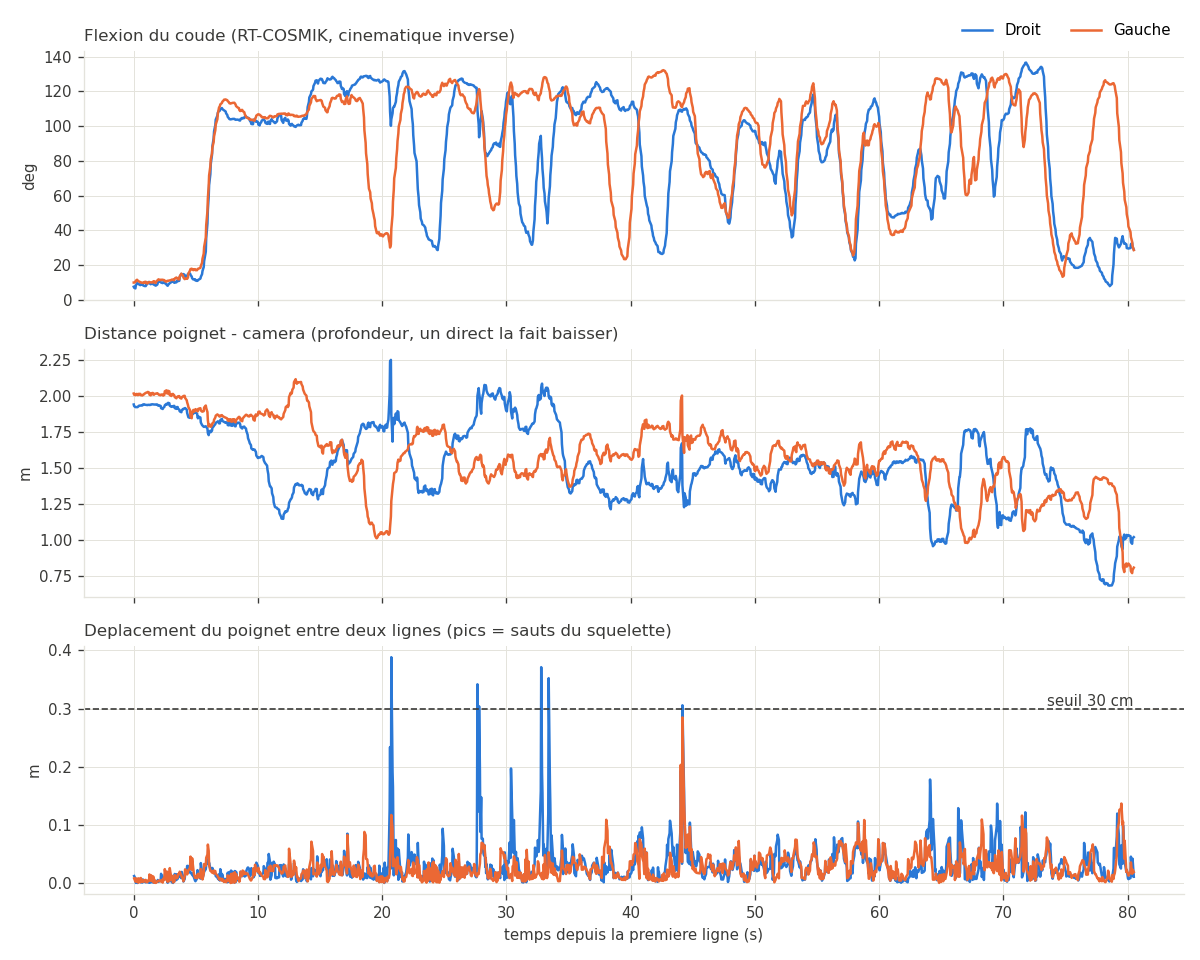
\includegraphics[width=\textwidth]{figures/analyse_demo03.png}
\caption{Prise \code{demo\_03}. En haut : flexion des coudes issue de la cinématique inverse (0° = bras tendu). Au milieu : distance poignet--caméra. En bas : déplacement du poignet entre deux lignes successives.}
\label{fig:analyse}
\end{figure}

\paragraph{Interprétation.}
\begin{itemize}
  \item Les données ont un sens physique. Coudes à environ 10° pendant la calibration (bras tendus), passage à environ 110° à la mise en garde vers 6~s, puis creux alternés gauche/droite entre 20 et 45~s correspondant aux directs.
  \item La profondeur suit les coups. À 20,5~s, l'ouverture du coude gauche coïncide avec un rapprochement du poignet gauche de la caméra (de 2~m à 1~m) : l'estimation monoculaire perçoit bien un coup dirigé vers l'objectif.
  \item Les proportions sont humaines et cohérentes avec un sujet de 1,73~m. Les avant-bras sont les moins stables, ce qui est attendu : ils sont devant le corps et dans l'axe de la caméra.
  \item Les \enquote{sauts} ont tous lieu pendant des coups. Une partie est réelle : un poignet en direct se déplace de plusieurs mètres par seconde, soit 30~cm entre deux images quand on n'a que 6 à 7 images réelles par seconde. C'est un sous-échantillonnage plus qu'une erreur.
  \item Cadrage : à 1,61~m, la caméra ne couvre que $2 \times 1{,}61 \times 240/f_y \approx 1{,}56$~m en hauteur, moins que la taille du sujet. Les pieds sont donc hors champ et les jambes en partie estimées par NLF. À 2,5~m, la couverture passe à 2,43~m.
\end{itemize}

% =============================================================================
\section{Limites actuelles et suite}
% =============================================================================

\begin{table}[H]
\centering
\begin{tabularx}{\textwidth}{@{}XX@{}}
\toprule
\textbf{Limite} & \textbf{Action prévue} \\
\midrule
6 à 13~fps réels (USB/IP sous WSL) ; un direct dure 1 à 2 images & \textcolor{vert}{\textbf{Résolu}} sur la Debian de Polytech : 30~images/s, toutes traitées \\
Une seule caméra : profondeur et occultations des bras & Deuxième caméra, angles de vue écartés de 45 à 90° (par exemple en haut et sur le côté du cadre du miroir), triangulation et calibration extrinsèque avec \code{cams\_calibration} \\
Repère monde approximatif (caméra supposée horizontale à 1,2~m) & Marqueur ArUco vu par la caméra de référence (\code{cam\_to\_world}) \\
Webcam de Polytech non calibrée (calibration UGREEN utilisée) & Calibration intrinsèque avec \code{calib\_intrinsics.py} \\
Filtre réglé pour 40~Hz (\code{system\_freq}) alors que la caméra tourne à 30~Hz & Aligner \code{system\_freq} sur la cadence réelle \\
Centre optique décalé de 41~px & Nouvelle calibration couvrant les bords de l'image \\
Synchronisation vidéo/CSV approximative & Horodatages communs caméra/capteurs (livrable~3) \\
Solveur \code{sbs} & Évaluer \code{mhe} (acados, profil \code{realtime}), plus lisse \\
\bottomrule
\end{tabularx}
\caption{Limites identifiées et actions correctives.}
\end{table}

\paragraph{Prochaines étapes.}
\begin{enumerate}
  \item Calibrer la webcam de Polytech et refaire l'analyse de qualité à 30~images/s.
  \item Vérifier TensorRT sur le PC Windows avec le même test (\code{trt.Builder}) et relancer le script de setup si besoin.
  \item Refaire une prise suivant le protocole (immobilité, garde, 5 directs lents par bras, bras en croix, coups rapides) à 2,5--3~m, bien éclairée.
  \item Ajouter la seconde caméra et la calibration extrinsèque.
  \item Démarrer le livrable 2 : choix des capteurs de pression, de l'électronique d'acquisition et de leur disposition derrière le miroir.
\end{enumerate}

\appendix
% =============================================================================
\section{Aide-mémoire : lancer une session}
% =============================================================================

\begin{lstlisting}[language=bash]
# Windows (PowerShell admin) : partager la webcam avec WSL
usbipd attach --wsl --busid 5-2
docker start 90034be366af
docker exec -it 90034be366af bash

# Conteneur
v4l2-ctl -d /dev/video0 -c exposure_dynamic_framerate=0
cd ~/workspace/ros_ws/RT-COSMIK-main
export YOLO_VERBOSE=False
python3 scripts/python/core/run_pipeline.py --online --cameras 0
# rester immobile jusqu'a "Model calibration finished", puis q et Ctrl+C

# Analyse de la prise
python3 analyze_take.py output/demo_03
bash overlay_offsets.sh output/demo_03 "0 0.5 1 1.5 2"
\end{lstlisting}

\section*{Session sur la machine Debian de Polytech}

\begin{lstlisting}[language=bash]
# Hote : autoriser l'affichage et entrer dans le conteneur
xhost +local: && docker start -ai cosmik

# Conteneur
cd ~/workspace/ros_ws/RT-COSMIK-main
YOLO_VERBOSE=False python3 scripts/python/core/run_pipeline.py --online --cameras 0

# Firefox sur l'hote : http://127.0.0.1:7000/static/
\end{lstlisting}

\section{Modifications apportées au code de RT-COSMIK}

\begin{lstlisting}
--- a/src/rtcosmik/nlf/nlf.py
+++ b/src/rtcosmik/nlf/nlf.py
@@ -1,5 +1,6 @@
 import numpy as np
 import torch
+import torchvision  # charge torchvision::nms, requis par le modele NLF (TorchScript)
 from ultralytics import YOLO
\end{lstlisting}

Patch \code{0003}, ajouté dans la boucle du processus pipeline (fichier \code{pipeline.py}) :

\begin{lstlisting}[language=Python]
if self.settings.show_video:
    # Same frame the skeleton was solved from, so the two stay in step.
    overlay = est.visualize_frames(frames, nlf_out, boxes=boxes,
                                   draw_boxes=True)
    cv2.imshow("RT-COSMIK cameras", np.hstack(overlay))
    cv2.waitKey(1)
\end{lstlisting}

\end{document}
